\documentclass[a4paper,10pt]{report}
\usepackage[utf8]{inputenc}
\usepackage{graphicx}
\usepackage[francais]{babel}

% Title Page
\title{Traveling Salesman Problem}
\author{Adrien DROGUET}
\date{Avril - Juin 2014}

\pagestyle{plain}

\begin{document}
\maketitle

\tableofcontents
\pagebreak

\section{Définitions}
\begin{itemize}
 \item Problème : Ensemble de villes devant être parcourues.
 \item Voisinage : Chemin parcourant toutes les villes sans répétition. Solution au problème du voyageur de commerce.
 \item Voisin améliorant : Chemin voisin d'une solution X, dont le coût est inférieur au coût de X.
 \item Recherche locale : Exploration exhaustive de l'ensemble des voisins d'une solution donnée.
 Couteux en temps d'exécution.
 \item Relation de voisinage : Fonction permettant de passer d'un voisnage à un autre.
 \begin{itemize}
  \item Swap : Échange la position de deux villes dans un chemin.
  \item Insert : Insert une ville avant une autre.
  \item Reverse : Inverse un sous section d'un chemin.
 \end{itemize}
 \item Stratégie de sélection : Détermine la manière dont on choisit un voisin en recherche locale.
 \begin{itemize}
  \item First Fit : Choisir le premier voisin améliorant trouvé.
  \item Best Fit : Choisir le meilleur améliorant trouvé.
  \item Worst Fit : Choisir le moins bon améliorant trouvé.
 \end{itemize}
\end{itemize}


\section{Introduction}

\paragraph{} % sujet
  Le voyageur de commerce est un problème bien connu dans le milieu informatique : pour un ensemble de villes,
minimiser la distance requise qu'un individu doit parcourir afin de visiter chaque ville. Le but de ce projet
est d'étudier l'efficacité de différents algorithmes et stratégies applicables à la résolution de ce problème
en recherce locale. Suite à l'étude des résultats de ces différents algos et stratégies, le projet vise la mise
en place de méthodes permettant d'effectuer une recherche partielle capable d'obtenir des résultats comparables
à ceux d'une recherche locale à un coût moindre en temps de calcul.

\paragraph{} % ressources utilisées
==> source des .tsp

%%%%%%%%%%%%%%%%%%%%
% Partie Recherche %
%%%%%%%%%%%%%%%%%%%%
\part{Recherche}
\chapter{Recherche locale}
\section{Implémentation des algorithmes}
\subsection{Relations de voisinage}

\paragraph{}
  Après avoir établit une représentation satisfaisante et un système de lecture des données fonctionnel (voir partie
développement, sous-section représentation des données), nous avons défini trois types de mouvements, ou relation de
voisinage à appliquer à une solution : l'échange (Swap), l'insertion (Insert) et l'inversion (Reverse).

\paragraph{}
Afin d'éviter de recalculer le coût d'une solution (c'est à dire la distance que le voyageur doit parcourir
pour un chemin donné), à chacune de ces relations est associé une fonction de calcul de coût potentielle.
Celle-ci prend en paramètre les villes sur lesquels seront appliqués les déplacements, et effectue les calculs
aux points de rupture du chemin modifié.
% insérer schéma types de déplacements + points de rupture
% reprendre comme exemple 0123456789


\subsection{Stratégies de sélection d'un voisinage}

\paragraph{}
  Une fois que l'on dispose d'une fonction permettant de calculer le voisinage d'une solution donnée, il faut déterminer
une stratégie d'amélioration à appliquer. Nous avons retenu trois stratégies distinctes à appliquer à notre recherche
locale : choisir le premier voisin améliorant que l'on trouve (First Fit), choisir le meilleur voisin améliorant après
avoir parcouru l'ensemble des voisins possibles (Best Fit), ou bien choisir le voisin améliorant le moins possible la
solution actuelle (Worst Fit).
% schémas d'exemples


\subsection{Lancement}

\paragraph{}
  Suite au parsage d'un TSP particulier, notre programme s'efforce d'appliquer chacune des relations et chacunes
des stratégies spécifiées l'une après l'autre, en partant éventuellement du même point de départ. Le voisinage de
départ est généré aléatoirement à partir des données du problème. Chaque pas est exploré de manière aléatoire, bien
que dans le cas des stratégies Best Fit et Worst Fit, on va chercher (dans un premier temps) à explorer l'ensemble
des voisins possibles.

\paragraph{}
En fin d'exécution, un résumé des résultats obtenus est affiché en console.
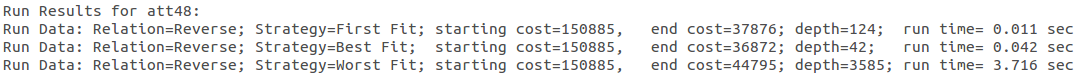
\includegraphics[width=\textwidth]{images/exec-summary.png} 

\section{Analyse et comparaison de l'efficacité des algos}
\subsection{Enregistrement des résultats}

\paragraph{}
  Après chaque exécution, on en enregistre les résultats dans des fichiers sous forme textuelle. On distingue deux
types de fichiers de sortie. D'une part les *.results sont équivalents à la sortie console en fin de programme et
fournissent un résumé facile à lire pour les humain.
\paragraph{}
  D'autre part, les *.csv contiennent les mêmes données enregistrées au format Comma Separated Value, ie. valeurs
séparées par virgule, chaque ligne correspondant à un couple Relation/Stratégie. Typiquement, le contenu de ces 
fichiers est concatené dans un fichier résumé, qui peut alors être copié tel quel dans un tableur type Microsoft
Excel ou Libre Office Calc. Voir en annexe pour description plus appronfondie du tableur utilisé.
  
% insérer extraits de .results et .csv
% insérer screen de recap.ods

\subsection{Efficacité constatée}
%Résultats
%insérer tableaux de stats à la place de la liste?
\begin{itemize}
 \item Swap - First Fit : 
 \item Swap - Best Fit : 
 \item Swap - Worst Fit : 
 \item Insert - First Fit :
 \item Insert - Best Fit :
 %...
\end{itemize}

%Conclusion

\chapter{Analyse d'efficacité \& espérance d'amélioration}

\paragraph{}
  Suite à l'étude prémliminaire de l'efficacité de chacun des relations et stratégies, on a cherché à étudier
plus en détail le comportement de ces algorithmes en cours d'exécution.

\section{Enregistrement du déroulement de l'algo pas à pas}

\paragraph{}
  Avant toute chose, il a fallu concevoir de nouvelles structures capable de représenter l'état de notre programme
à un instant t. Ensuite, ces classes ont été greffé au code existant sans en modifier le comportement. Finalement,
nous avons choisi d'enregistrer chaque étape, chaque ``pas'' ligne par ligne dans un fichier texte. Une fois encore,
nous utilisons le format .csv afin de pouvoir aisement transférer ces données dans un tableur au besoin.

\paragraph{}
  Via le tableur, nous avons pu établir des graphe retraçant l'historique de chaque exécution. La contrepartie de
cette méthode est la relative difficulté à comparer de nombreux résultats cote à cote, le logiciel n'étant pas
bien adapté pour traiter de tels volumes de données de manière dynamique.

\section{Analyse des résultats}

\section{Espérance d'amélioration - Implémentation d'un système de décision}

%%%%%%%%%%%%%%%%%%%%
% Partie technique %
%%%%%%%%%%%%%%%%%%%%
\part{Développement}
\chapter{Structure de l'application}
\section{Organisation des Classes}
\subsection{Représentation des données}
%core + parsage

\subsection{Compartimentalisation des algorithmes}
%relation & stratégie

\subsection{Exécution du programme}
%main, parser & runner

\subsection{Analyse Comportementale}
%interval stuff

\subsection{Recherche partielle}



\chapter{Déroulement du projet}
\section{Organisation}
\subsection{Standards auto-imposés}

\subsection{Gestion de version}

\subsection{Contrôle de non-régression}
%tests unitaires
%retro compatibilité

\subsection{Profiling et Optimisation}
%valgrind, callgrind & autre

\subsection{Optimisation}

\section{Difficultés techniques}

\end{document}          
